\documentclass{beamer}
\usepackage{amsmath,amssymb,animate,cancel,fourier,multirow,subfig,tikz,xcolor,xspace}
\usetikzlibrary{arrows,calc,backgrounds}
\beamertemplatenavigationsymbolsempty
\setbeamertemplate{bibliography item}[text]
\tikzstyle{na} = [baseline=-.5ex]
\usepackage{graphicx,caption}
\graphicspath{{img//},{Cahn-Hilliard//},{Ostwald_ripening//}}
\captionsetup{labelformat=empty,labelsep=none,font=footnotesize}
\usetheme{CambridgeUS}
\usecolortheme{orchid}
\usefonttheme{serif}
\useinnertheme{rectangles}
\title{MMSP Hackathon Results}
\author[Trevor Keller]{Trevor Keller, Jason Gruber$^*$, and Jonathan Guyer}
\institute[NIST MSED]{Materials Science and Engineering Division\\ National Institute of Standards and Technology\\ Gaithersburg, MD 20899\\$ $\\$^*$ (not from NIST)}
\date[CHiMaD PFM Workshop]{CHiMaD Phase Field Methods Hackathon \textbackslash\textbackslash\ Workshop}
\setcounter{tocdepth}{1}
\tikzset{>=latex}

\begin{document}
\begin{frame}
  \titlepage
\end{frame}

\begin{frame}{Simulation Software: MMSP}
 Mesoscale Microstructure Simulation Project (\url{github.com/mesoscale}), created by Jason Gruber: 
 templated classes in C++ for integrating parabolic PDEs. Now co-developed. Key features include:\\[\baselineskip]
 
 \vskip-\baselineskip
 \begin{itemize}
  \item \parbox{0.5\textwidth}{
	  Grid class in arbitrary dimensions with parallel domain decomposition and communication using MPI}\quad
	\begin{minipage}{0.4\textwidth}\centering
	  \includegraphics[width=0.8\textwidth]{GridClass}
	\end{minipage}
	\vskip\baselineskip
  \item \parbox{0.5\textwidth}{
	  Vector class, common format for multiple scalar fields ($\phi$,$c$,$T$)}\quad
	\begin{minipage}{0.4\textwidth}
	  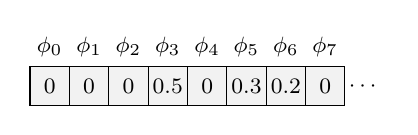
\begin{tikzpicture}[scale=0.5]
	    \foreach \x in {0,1,2,4,7} {
	      \begin{scope}[shift={(\x,0)}]
		\fill[black!10,opacity=.5] (0,0)-- (1,0)-- (1,1)-- (0,1) --cycle;
		\draw[] (0,0) -- (1,0) -- (1,1) -- (0,1) -- (0,0);
		\node at (0.5,1.5){\footnotesize{$\phi_\x$}};
		\node at (0.5,0.5){\footnotesize{$0$}};
	      \end{scope}
	    }
	    \begin{scope}[shift={(3,0)}]
	      \fill[black!10,opacity=.5] (0,0)-- (1,0)-- (1,1)-- (0,1) --cycle;
	      \draw[] (0,0) -- (1,0) -- (1,1) -- (0,1) -- (0,0);
	      \node at (0.5,1.5){\footnotesize{$\phi_3$}};
	      \node at (0.5,0.5){\footnotesize{$0.5$}};
	    \end{scope}
	    \begin{scope}[shift={(5,0)}]
	      \fill[black!10,opacity=.5] (0,0)-- (1,0)-- (1,1)-- (0,1) --cycle;
	      \draw[] (0,0) -- (1,0) -- (1,1) -- (0,1) -- (0,0);
	      \node at (0.5,1.5){\footnotesize{$\phi_5$}};
	      \node at (0.5,0.5){\footnotesize{$0.3$}};
	    \end{scope}
	    \begin{scope}[shift={(6,0)}]
	      \fill[black!10,opacity=.5] (0,0)-- (1,0)-- (1,1)-- (0,1) --cycle;
	      \draw[] (0,0) -- (1,0) -- (1,1) -- (0,1) -- (0,0);
	      \node at (0.5,1.5){\footnotesize{$\phi_6$}};
	      \node at (0.5,0.5){\footnotesize{$0.2$}};
	    \end{scope}
	    \begin{scope}[shift={(8,0)}]
	      \node at (0.5,0.5){\footnotesize{$\cdots$}};
	    \end{scope}
	  \end{tikzpicture}
	\end{minipage}
	\vskip\baselineskip
  \item \parbox{0.5\textwidth}{
	  Sparse vector class, storing the key-value pairs. Efficient access for multiorder-parameter models.\\
	  }\quad
	\begin{minipage}{0.4\textwidth}
	  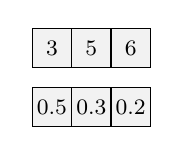
\begin{tikzpicture}[scale=0.5]
	    \begin{scope}[shift={(0,0)}]
	      \fill[black!10,opacity=.5] (0,0)-- (1,0)-- (1,-1)-- (0,-1) --cycle;
	      \draw[] (0,0) -- (1,0) -- (1,-1) -- (0,-1) -- (0,0);
	      \fill[black!10,opacity=.5] (0,-1.5)-- (1,-1.5)-- (1,-2.5)-- (0,-2.5) --cycle;
	      \draw[] (0,-1.5) -- (1,-1.5) -- (1,-2.5) -- (0,-2.5) -- (0,-1.5);
	      \node at (0.5,-0.5){\footnotesize{$3$}};
	      \node at (0.5,-2){\footnotesize{$0.5$}};
	    \end{scope}
	    \begin{scope}[shift={(1,0)}]
	      \fill[black!10,opacity=.5] (0,0)-- (1,0)-- (1,-1)-- (0,-1) --cycle;
	      \draw[] (0,0) -- (1,0) -- (1,-1) -- (0,-1) -- (0,0);
	      \fill[black!10,opacity=.5] (0,-1.5)-- (1,-1.5)-- (1,-2.5)-- (0,-2.5) --cycle;
	      \draw[] (0,-1.5) -- (1,-1.5) -- (1,-2.5) -- (0,-2.5) -- (0,-1.5);
	      \node at (0.5,-0.5){\footnotesize{$5$}};
	      \node at (0.5,-2){\footnotesize{$0.3$}};
	    \end{scope}
	    \begin{scope}[shift={(2,0)}]
	      \fill[black!10,opacity=.5] (0,0)-- (1,0)-- (1,-1)-- (0,-1) --cycle;
	      \draw[] (0,0) -- (1,0) -- (1,-1) -- (0,-1) -- (0,0);
	      \fill[black!10,opacity=.5] (0,-1.5)-- (1,-1.5)-- (1,-2.5)-- (0,-2.5) --cycle;
	      \draw[] (0,-1.5) -- (1,-1.5) -- (1,-2.5) -- (0,-2.5) -- (0,-1.5);
	      \node at (0.5,-0.5){\footnotesize{$6$}};
	      \node at (0.5,-2){\footnotesize{$0.2$}};
	    \end{scope}
	  \end{tikzpicture}
	\end{minipage} 
 \end{itemize}
 \footnotesize{Gruber, \emph{Modell. Simul. Mater. Sci. Eng.} \textbf{14} (2006) 1189.}
\end{frame}

\begin{frame}{MMSP Examples}
  \begin{minipage}{0.45\textwidth}
  	\begin{itemize}
  	\item beginners\_diffusion
  	\item coarsening
  	\begin{itemize}
	  \item grain\_growth
	  \item \textbf{ostwald\_ripening}
	  \item zener\_pinning
  	\end{itemize}
  	\item differential\_equations
  	\begin{itemize}
	  \item elliptic
	  \item stiff
  	\end{itemize}
  	
    \end{itemize}
  \end{minipage}
  \qquad
  \begin{minipage}{0.45\textwidth}
  \begin{itemize}
    \item phase\_transitions
  	\begin{itemize}
	  \item allen-cahn
	  \item \textbf{cahn-hilliard}
	  \item model\_A
	  \item model\_B
	  \item spinodal
  	\end{itemize}
  	\item solidification
  	\begin{itemize}
	  \item anisotropic
	  \item eutectic
  	\end{itemize}
  	\item statistical\_mechanics
  	\begin{itemize}
	  \item Heisenberg
	  \item ising
	  \item Potts
  	\end{itemize}
  \end{itemize}
  \end{minipage}  
\end{frame}

\begin{frame}{Hardware}
	Code was executed remotely on an 8-socket Opteron workstation:\\ 64 cores at 3GHz and with 256GB RAM.
\end{frame}


\begin{frame}
	\large{1. Spinodal Decomposition}
\end{frame}

\begin{frame}{Code, using $\vec{q}=(0.1\sqrt{2},0.1\sqrt{3})$}
	\includegraphics[height=\textheight]{cahncode}
\end{frame}

\begin{frame}{1A: Energy}\centering
  Spinodal decomposition with periodic boundary conditions
  
	\includegraphics[height=0.8\textheight]{{1a_Periodic/energy}}
\end{frame}
\begin{frame}{1A: Init}\centering
	\includegraphics[height=0.8\textheight]{{1a_Periodic/img/cahn_0000000}}
	
	$\Delta t=0.005 \rightarrow CFL=0.01$
\end{frame}
\begin{frame}{1A: Evolution, $250k \Delta t$}\centering
	\includegraphics[height=0.8\textheight]{{1a_Periodic/img/cahn_0250000}}
\end{frame}
\begin{frame}{1A: Evolution, $500k \Delta t$}\centering
	\includegraphics[height=0.8\textheight]{{1a_Periodic/img/cahn_0500000}}
\end{frame}
\begin{frame}{1A: Evolution, $750k \Delta t$}\centering
	\includegraphics[height=0.8\textheight]{{1a_Periodic/img/cahn_0750000}}
\end{frame}
\begin{frame}{1A: Evolution, $1000k \Delta t$}\centering
	\includegraphics[height=0.8\textheight]{{1a_Periodic/img/cahn_1000000}}
\end{frame}
\begin{frame}{1A: Evolution, $1250k \Delta t$}\centering
	\includegraphics[height=0.8\textheight]{{1a_Periodic/img/cahn_1250000}}
\end{frame}
\begin{frame}{1A: Evolution, $1500k \Delta t$}\centering
	\includegraphics[height=0.8\textheight]{{1a_Periodic/img/cahn_1500000}}
	
	Runtime to steady state: 1 hour (wall), 64 CPU-hours.
\end{frame}

\begin{frame}{1B: Energy}\centering
  Spinodal decomposition with Neumann boundary conditions
  
	\includegraphics[height=0.8\textheight]{{1b_Neumann/energy}}
\end{frame}
\begin{frame}{1B: Init}\centering
	\includegraphics[height=0.8\textheight]{{1b_Neumann/img/cahn_0000000}}
	
	$\Delta t=0.005 \rightarrow CFL=0.01$
\end{frame}
\begin{frame}{1B: Evolution, $250k \Delta t$}\centering
	\includegraphics[height=0.8\textheight]{{1b_Neumann/img/cahn_0250000}}
\end{frame}
\begin{frame}{1B: Evolution, $500k \Delta t$}\centering
	\includegraphics[height=0.8\textheight]{{1b_Neumann/img/cahn_0500000}}
\end{frame}
\begin{frame}{1B: Evolution, $750k \Delta t$}\centering
	\includegraphics[height=0.8\textheight]{{1b_Neumann/img/cahn_0750000}}
\end{frame}
\begin{frame}{1B: Evolution, $1000k \Delta t$}\centering
	\includegraphics[height=0.8\textheight]{{1b_Neumann/img/cahn_1000000}}
\end{frame}
\begin{frame}{1B: Evolution, $1250k \Delta t$}\centering
	\includegraphics[height=0.8\textheight]{{1b_Neumann/img/cahn_1250000}}
\end{frame}
\begin{frame}{1B: Evolution, $1500k \Delta t$}\centering
	\includegraphics[height=0.8\textheight]{{1b_Neumann/img/cahn_1500000}}
\end{frame}
\begin{frame}{1B: Evolution, $1750k \Delta t$}\centering
	\includegraphics[height=0.8\textheight]{{1b_Neumann/img/cahn_1750000}}
\end{frame}
\begin{frame}{1B: Evolution, $2000k \Delta t$}\centering
	\includegraphics[height=0.8\textheight]{{1b_Neumann/img/cahn_2000000}}
	
	Runtime to steady state: 80 minutes (wall), 85 CPU-hours.
\end{frame}


\begin{frame}{1C: Code}\centering
  Spinodal decomposition on T-square domain with Neumann boundary conditions
  
	\includegraphics[height=0.8\textheight]{{tlap}}
\end{frame}
\begin{frame}{1C: Energy}\centering
  Spinodal decomposition on T-square domain with Neumann boundary conditions
  
	\includegraphics[height=0.8\textheight]{{1c_Tsquare/energy}}
\end{frame}
\begin{frame}{1C: Init}\centering
	\includegraphics[height=0.8\textheight]{{1c_Tsquare/img/cahn_000000}}
	
	$\Delta t=0.005 \rightarrow CFL=0.01$
\end{frame}
\begin{frame}{1C: Evolution, $100 \Delta t$}\centering
	\includegraphics[height=0.8\textheight]{{1c_Tsquare/img/cahn_100000}}
\end{frame}
\begin{frame}{1C: Evolution, $200 \Delta t$}\centering
	\includegraphics[height=0.8\textheight]{{1c_Tsquare/img/cahn_200000}}
\end{frame}
\begin{frame}{1C: Evolution, $300 \Delta t$}\centering
	\includegraphics[height=0.8\textheight]{{1c_Tsquare/img/cahn_300000}}
\end{frame}
\begin{frame}{1C: Evolution, $400k \Delta t$}\centering
	\includegraphics[height=0.8\textheight]{{1c_Tsquare/img/cahn_400000}}
\end{frame}
\begin{frame}{1C: Evolution, $500k \Delta t$}\centering
	\includegraphics[height=0.8\textheight]{{1c_Tsquare/img/cahn_500000}}
	
	Runtime to steady state: 9 minutes (wall), 10 CPU-hours.
\end{frame}
\begin{frame}{1D: Sphere}\centering
  Rectilinear grids, only: spherical geometries are not accessible to MMSP.
\end{frame}
\begin{frame}{1E: Energy}\centering
  Spinodal decomposition with periodic boundary conditions, refined grid
  
	\includegraphics[height=0.8\textheight]{{1e_refine/energy}}
\end{frame}
\begin{frame}{1A: Init}\centering
	\includegraphics[height=0.8\textheight]{{1e_refine/img/cahn_00000000}}
	
	$\Delta t=0.001 \rightarrow CFL\approx0.01$
\end{frame}
\begin{frame}{1E: Evolution, $1000k \Delta t$}\centering
	\includegraphics[height=0.8\textheight]{{1e_refine/img/cahn_01000000}}
\end{frame}
\begin{frame}{1E: Evolution, $2000k \Delta t$}\centering
	\includegraphics[height=0.8\textheight]{{1e_refine/img/cahn_02000000}}
\end{frame}
\begin{frame}{1E: Evolution, $3000k \Delta t$}\centering
	\includegraphics[height=0.8\textheight]{{1e_refine/img/cahn_03000000}}
\end{frame}
\begin{frame}{1E: Evolution, $4000k \Delta t$}\centering
	\includegraphics[height=0.8\textheight]{{1e_refine/img/cahn_04000000}}
\end{frame}
\begin{frame}{1E: Evolution, $5000k \Delta t$}\centering
	\includegraphics[height=0.8\textheight]{{1e_refine/img/cahn_05000000}}
	
	Runtime to steady state: unknown. 5 million steps took 7 hours (wall).
\end{frame}



\begin{frame}
	2. Ostwald ripening
\end{frame}

\begin{frame}{Code, using $\vec{q}=(\sqrt{2},\sqrt{3})$, $\vec{q}_i=(0.01\sqrt{23+i},0.01\sqrt{149+i})$}\centering
	\includegraphics[height=\textheight]{ostwaldcode}
\end{frame}
\begin{frame}{2A: Energy}\centering
  Ostwald ripening with periodic boundary conditions
  
	\includegraphics[height=0.8\textheight]{{2a_Periodic/energy}}
\end{frame}
\begin{frame}{2A: Initial Condition}\centering
	\centerline{concentration\hspace{0.25\textwidth} magnitude of order}
	
	\includegraphics[height=0.45\textwidth]{{2a_Periodic/img/ostwald_000000}}\quad
	\includegraphics[height=0.45\textwidth]{{2a_Periodic/img/ostwald_000000_p}}
	
	$\Delta t=0.005 \rightarrow CFL=0.01$
\end{frame}
\begin{frame}{2A: Evolution, $20k \Delta t$}\centering
	\centerline{concentration\hspace{0.25\textwidth} magnitude of order}
	
	\includegraphics[height=0.45\textwidth]{{2a_Periodic/img/ostwald_020000}}\quad
	\includegraphics[height=0.45\textwidth]{{2a_Periodic/img/ostwald_020000_p}}
\end{frame}
\begin{frame}{2A: Evolution, $50k \Delta t$}\centering
	\centerline{concentration\hspace{0.25\textwidth} magnitude of order}
	
	\includegraphics[height=0.45\textwidth]{{2a_Periodic/img/ostwald_050000}}\quad
	\includegraphics[height=0.45\textwidth]{{2a_Periodic/img/ostwald_050000_p}}
\end{frame}
\begin{frame}{2A: Evolution, $100k \Delta t$}\centering
	\centerline{concentration\hspace{0.25\textwidth} magnitude of order}
	
	\includegraphics[height=0.45\textwidth]{{2a_Periodic/img/ostwald_100000}}\quad
	\includegraphics[height=0.45\textwidth]{{2a_Periodic/img/ostwald_100000_p}}
\end{frame}
\begin{frame}{2A: Evolution, $150k \Delta t$}\centering
	\centerline{concentration\hspace{0.25\textwidth} magnitude of order}
	
	\includegraphics[height=0.45\textwidth]{{2a_Periodic/img/ostwald_150000}}\quad
	\includegraphics[height=0.45\textwidth]{{2a_Periodic/img/ostwald_150000_p}}
	
	Runtime to steady state: 174 minutes (wall), 185 CPU-hours.
\end{frame}

\begin{frame}{2B: Energy}\centering
  Ostwald ripening with Neumann boundary conditions
  
	\includegraphics[height=0.8\textheight]{{2b_Neumann/energy}}
\end{frame}
\begin{frame}{2B: Initial Condition}
	\centerline{concentration\hspace{0.25\textwidth} magnitude of order}
	
	\includegraphics[height=0.45\textwidth]{{2b_Neumann/img/ostwald_000000}}\quad
	\includegraphics[height=0.45\textwidth]{{2b_Neumann/img/ostwald_000000_p}}
	
	$\Delta t=0.005 \rightarrow CFL=0.01$
\end{frame}
\begin{frame}{2B: Evolution, $20k \Delta t$}\centering
	\centerline{concentration\hspace{0.25\textwidth} magnitude of order}
	
	\includegraphics[height=0.45\textwidth]{{2b_Neumann/img/ostwald_020000}}\quad
	\includegraphics[height=0.45\textwidth]{{2b_Neumann/img/ostwald_020000_p}}
\end{frame}
\begin{frame}{2B: Evolution, $50k \Delta t$}\centering
	\centerline{concentration\hspace{0.25\textwidth} magnitude of order}
	
	\includegraphics[height=0.45\textwidth]{{2b_Neumann/img/ostwald_050000}}\quad
	\includegraphics[height=0.45\textwidth]{{2b_Neumann/img/ostwald_050000_p}}
\end{frame}
\begin{frame}{2B: Evolution, $100k \Delta t$}\centering
	\centerline{concentration\hspace{0.25\textwidth} magnitude of order}
	
	\includegraphics[height=0.45\textwidth]{{2b_Neumann/img/ostwald_100000}}\quad
	\includegraphics[height=0.45\textwidth]{{2b_Neumann/img/ostwald_100000_p}}
\end{frame}
\begin{frame}{2B: Evolution, $150k \Delta t$}\centering
	\centerline{concentration\hspace{0.25\textwidth} magnitude of order}
	
	\includegraphics[height=0.45\textwidth]{{2b_Neumann/img/ostwald_150000}}\quad
	\includegraphics[height=0.45\textwidth]{{2b_Neumann/img/ostwald_150000_p}}
	
	Runtime to steady state: 181 minutes (wall), 193 CPU-hours.
\end{frame}

\begin{frame}{2C: Energy}\centering
  Ostwald ripening with Neumann boundary conditions
  
	\includegraphics[height=0.8\textheight]{{2c_Tsquare/energy}}
\end{frame}
\begin{frame}{2C: Initial Condition}\centering
	\centerline{concentration\hspace{0.25\textwidth} magnitude of order}
	
	\includegraphics[height=0.45\textwidth]{{2c_Tsquare/img/ostwald_0000000}}\quad
	\includegraphics[height=0.45\textwidth]{{2c_Tsquare/img/ostwald_0000000_p}}
	
	$\Delta t=0.005 \rightarrow CFL=0.01$
\end{frame}
\begin{frame}{2C: Evolution, $20k \Delta t$}\centering
	\centerline{concentration\hspace{0.25\textwidth} magnitude of order}
	
	\includegraphics[height=0.45\textwidth]{{2c_Tsquare/img/ostwald_0020000}}\quad
	\includegraphics[height=0.45\textwidth]{{2c_Tsquare/img/ostwald_0020000_p}}
\end{frame}
\begin{frame}{2C: Evolution, $50k \Delta t$}\centering
	\centerline{concentration\hspace{0.25\textwidth} magnitude of order}
	
	\includegraphics[height=0.45\textwidth]{{2c_Tsquare/img/ostwald_0050000}}\quad
	\includegraphics[height=0.45\textwidth]{{2c_Tsquare/img/ostwald_0050000_p}}
\end{frame}
\begin{frame}{2C: Evolution, $100k \Delta t$}\centering
	\centerline{concentration\hspace{0.25\textwidth} magnitude of order}
	
	\includegraphics[height=0.45\textwidth]{{2c_Tsquare/img/ostwald_0100000}}\quad
	\includegraphics[height=0.45\textwidth]{{2c_Tsquare/img/ostwald_0100000_p}}
\end{frame}
\begin{frame}{2C: Evolution, $150k \Delta t$}\centering
	\centerline{concentration\hspace{0.25\textwidth} magnitude of order}
	
	\includegraphics[height=0.45\textwidth]{{2c_Tsquare/img/ostwald_0150000}}\quad
	\includegraphics[height=0.45\textwidth]{{2c_Tsquare/img/ostwald_0150000_p}}
	
	Runtime to steady state: 114 minutes (wall), 122 CPU-hours.
\end{frame}
 \begin{frame}{2D: Sphere}
  Rectilinear grids, only: spherical geometries are not accessible to MMSP.
\end{frame}


\end{document}
